%%This is a very basic article template.
%%There is just one section and two subsections.
%\documentclass[12pt,oneside,a4paper,doublespacing]{article} % for submission
\documentclass[11pt,oneside,a4paper]{article} % for sharing
\usepackage{apacite}
\usepackage{appendix}
\usepackage{amsmath}
\usepackage{caption}
\usepackage{placeins}
\usepackage{graphicx}
\usepackage{subcaption}
%\usepackage{subfig}
\usepackage{longtable}
\usepackage{setspace}
%\usepackage{tikz}
\usepackage{booktabs}
\usepackage{tabularx}
\usepackage{xcolor,colortbl}
\usepackage{chngpage}
%\usepackage[active,tightpage]{preview}
\usepackage{natbib}
\bibpunct{(}{)}{,}{a}{}{;} 
\usepackage{url}
\usepackage{nth}
\usepackage{authblk}
\usepackage[most]{tcolorbox}
%\usepackage{hyperref}
%\usepackage{color}
%\usepackage{fontspec}
%\usepackage{pdfsync}
\usepackage[normalem]{ulem}
\usepackage{amsfonts}
%\renewcommand{\listtablename}{List of Appendix Tables}
\newcolumntype{C}[1]{>{\centering\let\newline\\\arraybackslash\hspace{0pt}}m{#1}}
\newcolumntype{L}[1]{>{\raggedright\let\newline\\\arraybackslash\hspace{0pt}}m{#1}}
% working on this need to concatenate file name based on sex and variable name
%\newcommand\Cell[1]{{\raisebox{-0.05in}{\includegraphics[height=.2in,width=.2in]{Figures/ColorCodes/\expandafter#1}}}}  

% for Demography submission: floats at the end.
%\usepackage{endfloat}
% otherwise it ignores this big table!
%\DeclareDelayedFloatFlavour*{longtable}{table}
\usepackage[margin=1in]{geometry}
%\doublespacing % for review

% line numbers to make review easier
%\usepackage{lineno}
%\linenumbers
%%%%%%%%%%%%%%%%%%%%%%%%%%%%%%%%%%%%%%%%%%%%%%%%%%%%%%%%%%%%%%%%%%%%%%%%%%%%%
% setting color to letters affects spacing. Here's a hack I found here:
% http://tex.stackexchange.com/questions/212736/change-letter-colour-without-losing-letter-spacing
%\DeclareRobustCommand{\spacedallcaps}[1]{\MakeUppercase{\textsc{#1}}} % all
% caps with better spacing

%\colorlet{RED}{red}
%\colorlet{BLUE}{b}
\colorlet{rd}{red}
\colorlet{bl}{blue}

%%%%%%%%%%%%%%%%%%%%%%%%%%%%%%%%%%%%%%%%%%%%%%%%%%%%%%%%%%%%%%%%%%%%%%%%%%%%%%

\newcommand\ackn[1]{%
  \begingroup
  \renewcommand\thefootnote{}\footnote{#1}%
  \addtocounter{footnote}{-1}%
  \endgroup
}
\newcommand\vt[1]{\textcolor{rd}{#1}}
\newcommand\eg[1]{\textcolor{bl}{#1}}

\newcommand\tg[1]{\includegraphics[scale=.5]{Figures/triadtable/triad#1.pdf}}
\newcommand\tgh[1]{\raisebox{-.25\height}{\includegraphics[scale=.3]{Figures/triadtable/triad#1.pdf}}}

\defcitealias{HMD}{HMD}

% junk for longtable caption
\AtBeginEnvironment{longtable}{\linespread{1}\selectfont}
\setlength{\LTcapwidth}{\linewidth}

%%%%%%%%%%%%%%%%%%%%%%%%%%%%%%%
\begin{document}

\title{A unified framework of demographic time}
%\author{author(s) redacted}
\author[1]{Tim Riffe\thanks{riffe@demogr.mpg.de}}
\author[2,3]{Jonas Sch{\"o}ley}
\author[2,3]{Francisco Villavicencio}
\affil[1]{Max Planck Institute for Demographic Research}
\affil[2]{University of Southern Denmark}
\affil[3]{Max-Planck Odense Center on the Biodemography of Aging}

\maketitle
\vspace{1em}
(Most sections omitted for brevity of abstract. In these
sections vocabulary is developed, and the full relationship is derived
bottom-up. Several new diagrams are introduced. Discussion and conclusions also
omitted. A complete paper is available on request (currently under review))

\section*{Introduction}
%\sout{so-called} \textbf{well-known?} 
In the course of training, all demographers are introduced
to the Lexis diagram, a convenient graphical identity between the three main
time measures used to structure demographic stocks and flows: Age, period, and birth cohort.
This popular representation does not account for remaining years of life and
other related time indices that may be of interest to researchers and
policy makers. % The Lexis diagram relates the chronological age (A), period (P),
% and birth cohort (C) measures of demographic time, APC, but it does not account
% for remaining years of life (thanatological age), and other related time
% indices.

We wish to draw attention to three time indices that are complementary to age
(A), period (P) and birth cohort (C). The first such index is time-to-death,
which we refer to as ``thanatological age'' (T) in contrast to ``chronological
age'' (A). The second index is death cohort (D), which groups all individuals
(of different ages) dying in the same time period. Finally, lifespan (L) or
age-at-death itself is an index by which data may be structured.
We therefore have six time measures in total to relate. We call these measures of demographic
time because each, except period, depends on the timing of birth, death, or
both.

Just as the Lexis diagram has been a fundamental instrument to
teach demography for decades, we hope that the demographic time measures and
their graphical depictions presented here will be helpful to teachers and
young demographers. The temporal relationships we describe will also be useful
for researchers to better understand the temporal structure of data, and for methodologists to
better account for the temporal structure of data in demographic methods.

The Lexis diagram can be understood as an APC plane
that relates age (A), period (P), and birth cohort (C). Other such planes also
exist. The ``thanatological'' counterpart to APC is an identity between
thanatological age (T), period (P), and death cohort (D), TPD. A third identity
relates thanatological age (T), chronological age (A), and lifespan (L), TAL. Finally, a potentially less
intuitive graphical identity relates lifespan (L), birth cohort (C), and death
cohort (D), LCD. We call three-way identities of this sort ``triad identities''.
% The thanatological counterpart to APC is an identity between thanatological
% age (T), period (P), and death cohort (D), TPD. A third
% identity exists between thanatological age (T), chronological age (A), and
% lifespan (L), TAL, and a fourth between lifespan (L), year of birth (C) and year
% of death (D), LCD.

Each of these four triad identities (APC, TPD, TAL, and LCD) may be sufficiently described by any two of its constituent indices, making the third index redundant. For instance, if the age (A) of an individual in a particular time period (P) is known, the birth cohort (C) to which he or she belongs can be immediately derived. Moreover, each of these four identities also lacks a major dimension of time. The TAL identity lacks calendar time, the LCD identity is ageless, APC lacks an endpoint in time, and TPD lacks a starting point in time.
% Each of these four identities may be sufficiently described by any
% two of its consituent indices, making the third index redundant. Each of these
% four identities also lacks a major dimension of time. The TAL identity
% lacks calendar time, the LCD identity is ageless, APC lacks an endpoint in time,
% and TPD lacks a starting point in time. We refer to these four identities
% as the triad identities.
To our knowledge, the only triad identity that has received serious
treatment at the time of this writing is the APC identity. Different
aspects of the APC identity have been discussed since at least 1868
\citep{knapp1868ermittlung}, and discussion remains lively today. Here we relate the six major indices of time in a geometric identity, in much the same spirit as the work on APC relationships done between the late
1860s and mid 1880s.\footnote{See e.g., \citet{keiding2011age} for an overview of that literature.} 

The objective of this paper is to describe the geometric identity between all
six measures of demographic time, a hexad identity, that may be useful or an intuitive
referent for demographers in the same way as the Lexis diagram. At the same time, this identity relates the
four triad identities we have mentioned. We give a bottom-up
description of how the six dimensions of time relate in a single framework,
building from familiar components to the full relationship.
We begin by defining some terms used throughout the manuscript. We then explore all combinations of two time
measures, the dyadic relationships, followed by the four triad identities, and
finally the hexad identity. We give a systematic topological overview of the
different elements of demographic time. 

%This paper contains no data visualizations, but it may serve as a basis for designing some.
 \section*{Diagram of the hexad identity}
 There are different ways to proportion this three dimensional construct,
of which we only present the isotropric mapping. In an isotropic projection, the
tetrahedron is regular, such that all edges are of the same length, and the
units of each of the six time measures are proportional. In this case, the four triad identities are based on equilateral triangles between their three constituent indices, and the four planes are joined together such that each is parallel to a face from the regular
tetrahedron. If the plane parallel to each face is repeated in equal
intervals and in parallel fashion, we create an isotropic 3d space.

In geometric nomenclature, the isotropic 3d space that results from this
framework is called the tetrahedral-octahedral honeycomb, a kind of
space-filling tessellation. Constructs following this geometry exist in nature, in other
theoretical settings, and in man-made structures. There are
various ways in which one might diagram or visualize the 3d space of demographic
time according to this geometric construct. Displaying all planes simultaneously
creates a very dense and difficult-to-read figure. We choose instead to
emphasize particular planes and intersections. 

In Fig.~\ref{fig:apctTAL} we
offer a view of the hexad identity, where birth-cohort TAL cross-sectional
planes are placed in sequence in a perspective drawing.\footnote{The coordinates
used to generate Figures~\ref{fig:apctTAL} and \ref{fig:apctAPC} are isotropic.
However, there are no 60$^\circ$ angles in this figure due to the use of parallax and an indirect viewing angle in this rendering for the sake of increased legibility.} The most recent TAL plane, for year $t$, is placed in the front, whereas past TAL planes are stacked behind it, highlighted in century intervals.
This view emphasizes how the juxtaposition of thanatological age,
chronological age, and lifespan shifts over time. This is the view used in
\citet{riffe2015ttd} to describe late-life health outcomes, albeit for a single
birth cohort.
The base of this figure is the APC plane, drawn for thanatological age 0. Each
of the TAL planes therefore sits atop a single birth cohort line from the APC plane that makes up the base of the
figure. 

\begin{figure}[!h]
\centering
%\begin{adjustwidth}{-2em}{-2em}
\caption[cap]{Birth cohort TAL planes over time}
\label{fig:apctTAL}
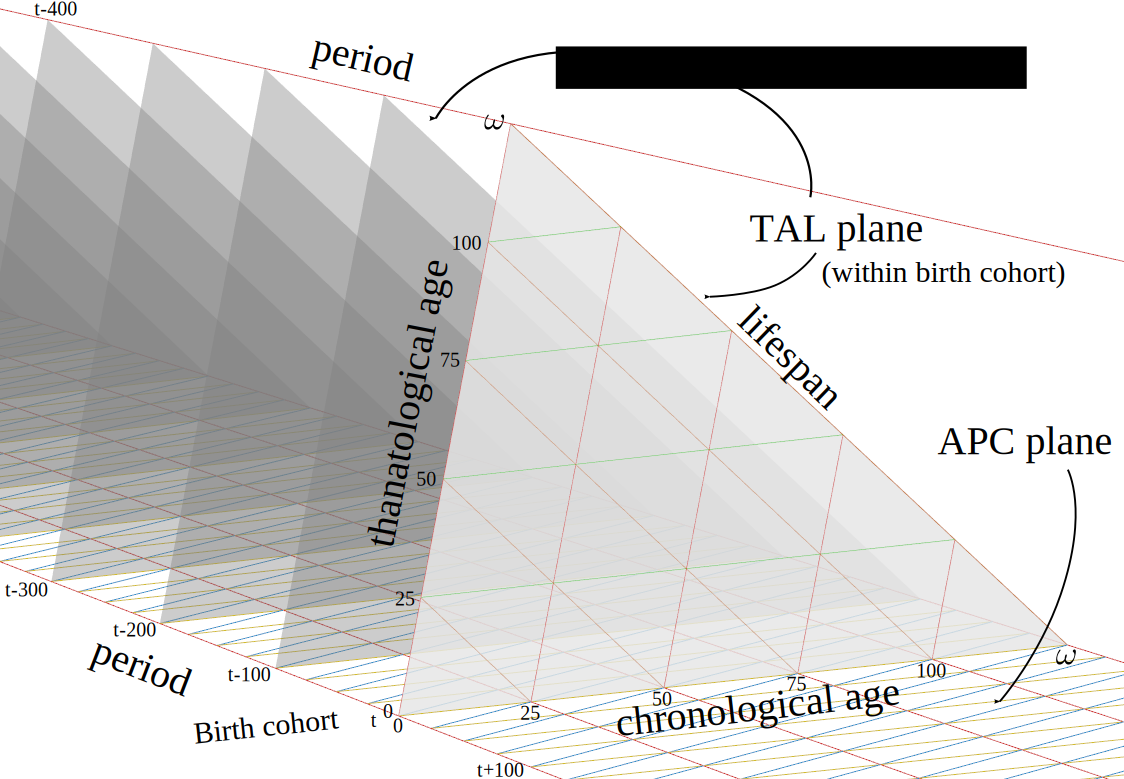
\includegraphics[scale=.5]{Figures/TALisomarkedup.pdf}
%\end{adjustwidth}
\end{figure}

Since the APC plane at the base of Fig.~\ref{fig:apctTAL} could have been
drawn for any thanatological age, it is better to imagine the TAL plane slicing
through the same birth cohort, $t$, of every possible thanatological APC plane.
In Fig.~\ref{fig:apctAPC} we gaze from a different angle and highlight
different planes to emphasize how the APC planes stack by thanatological age. The space in
this view is capped by period TAL planes on either side. Think of period TAL
planes as population censuses that have been fully linked to
mortality outcomes, such that each person is categorized by thanatological
age as well as chronological age (and each of the other indices). Period
TAL planes shift over time, like the birth
cohort TAL planes in Fig.~\ref{fig:apctTAL}, but the period and cohort TAL
planes stand in intersection.

\begin{figure}[!h]
\centering
\begin{adjustwidth}{-6em}{-6em}
\caption[cap]{The APC plane of thanatological age 25, with period TAL planes.}
\label{fig:apctAPC}
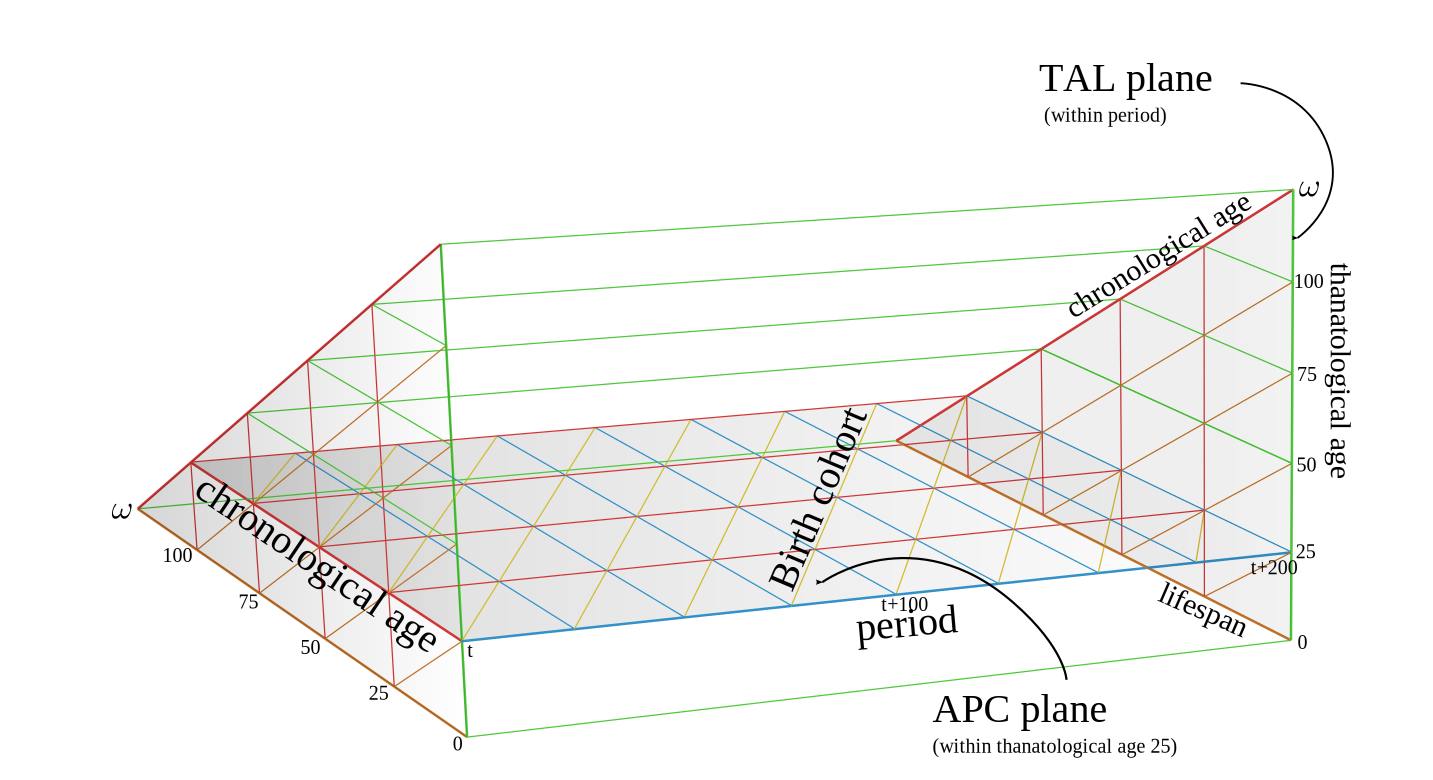
\includegraphics[scale=.5]{Figures/APCisomarkedup.pdf}
\end{adjustwidth}
\end{figure}

The APC shown in Fig.~\ref{fig:apctAPC} is drawn for thanatological age 25,
but we can think of it as shifting up and down through the space.
At the peak, near $\omega$ remaining years of life, the age axis of the plane is short, since
only the lowest chronological ages may live so long. The APC base plane at
thanatological age 0 is the largest because members of any chronological may
die.
\FloatBarrier

\bibliographystyle{apacite} % required for demography
  \bibliography{references} 


\end{document}